%% abtex2-modelo-artigo.tex, v-1.9.7 laurocesar
%% Copyright 2012-2018 by abnTeX2 group at http://www.abntex.net.br/ 
%%
%% This work may be distributed and/or modified under the
%% conditions of the LaTeX Project Public License, either version 1.3
%% of this license or (at your option) any later version.
%% The latest version of this license is in
%%   http://www.latex-project.org/lppl.txt
%% and version 1.3 or later is part of all distributions of LaTeX
%% version 2005/12/01 or later.
%%
%% This work has the LPPL maintenance status `maintained'.
%% 
%% The Current Maintainer of this work is the abnTeX2 team, led
%% by Lauro César Araujo. Further information are available on 
%% http://www.abntex.net.br/
%%
%% This work consists of the files abntex2-modelo-artigo.tex and
%% abntex2-modelo-references.bib
%%
% ---------------------------------------------------------------
% ---------------------------------------------------------------
% abnTeX2: Modelo de Artigo Acadêmico em conformidade com
% ABNT NBR 6022:2018: Informação e documentação - Artigo em publicação 
% periódica científica - Apresentação
% ---------------------------------------------------------------
% Adaptado para uso na instituição acadêmica Senai Cimatec.
% 25/05/2022
% -----------------------------------------------------------------

\documentclass[
	% -- opções da classe memoir --
	article,			% indica que é um artigo acadêmico
	11pt,				% tamanho da fonte
	oneside,			% para impressão apenas no recto. Oposto a twoside
	a4paper,			% tamanho do papel. 
	% -- opções da classe abntex2 --
	%chapter=TITLE,		% títulos de capítulos convertidos em letras maiúsculas
	%section=TITLE,		% títulos de seções convertidos em letras maiúsculas
	%subsection=TITLE,	% títulos de subseções convertidos em letras maiúsculas
	%subsubsection=TITLE % títulos de subsubseções convertidos em letras maiúsculas
	% -- opções do pacote babel --
	english,			% idioma adicional para hifenização
	brazil,				% o último idioma é o principal do documento
	sumario=tradicional
	]{abntex2}

% --- Pacotes fundamentais 
\usepackage{lmodern}		% Usa a fonte Latin Modern
\usepackage[T1]{fontenc}	% Selecao de codigos de fonte.
\usepackage[utf8]{inputenc}	% Conversão automática dos acentos
\usepackage{indentfirst}	% Indenta o 1. parágrafo de cada seção.
\usepackage{nomencl} 		% Lista de simbolos
\usepackage{color}			% Controle das cores
\usepackage{xcolor}         % Criação de label com cores específicas
\usepackage{graphicx}		% Inclusão de gráficos
\usepackage{microtype} 		% para melhorias de justificação
% --- Pacotes extras
\usepackage{lipsum}			% para geração de dummy text
% --- Pacotes de citações
\usepackage[brazilian,hyperpageref]{backref}	
\usepackage[alf]{abntex2cite}

\usepackage{tikz} % Pacotes para manipulação de imagens
\usepackage{float} % habilita a opção [H] (here) nas imagens
\usepackage{listings} % inserção de código no PDF

% ---
% Configurações do pacote listings

% criação de cores personalizadas
\definecolor{gray}{RGB}{160, 161, 167}
\definecolor{yellow}{RGB}{197, 163, 50}
\definecolor{backcolour}{RGB}{249, 249, 249}
\definecolor{blu}{RGB}{0, 152, 221}

% configurações de estilo personalizado para o pacote listing
\lstdefinestyle{bluloco-light}{
    backgroundcolor=\color{backcolour},   
    commentstyle=\itshape\color{gray},
    keywordstyle=\bfseries\color{blu},
    numberstyle=\tiny\color{gray},
    stringstyle=\color{yellow},
    basicstyle=\ttfamily\footnotesize,
    breakatwhitespace=false,
    breaklines=true,                 
    captionpos=b,                    
    keepspaces=true,                 
    numbers=left,                    
    numbersep=5pt,                  
    showspaces=false,                
    showstringspaces=false,
    showtabs=false,                  
    tabsize=2
}

% definição do estilo do pacote listing
\lstset{style=bluloco-light}

%//todo o que quem dizer isso? porque? é necessário fazer comentários.
%//valar erick suzart
%//checked mhar-vell OK

% mapeamento de caracteres especiais: necessário para adicionar caracteres
% especiais em código utilizando o pacote listing
\lstset{literate=
  {á}{{\'a}}1 {é}{{\'e}}1 {í}{{\'i}}1 {ó}{{\'o}}1 {ú}{{\'u}}1
  {Á}{{\'A}}1 {É}{{\'E}}1 {Í}{{\'I}}1 {Ó}{{\'O}}1 {Ú}{{\'U}}1
  {à}{{\`a}}1 {è}{{\`e}}1 {ì}{{\`i}}1 {ò}{{\`o}}1 {ù}{{\`u}}1
  {À}{{\`A}}1 {È}{{\'E}}1 {Ì}{{\`I}}1 {Ò}{{\`O}}1 {Ù}{{\`U}}1
  {ä}{{\"a}}1 {ë}{{\"e}}1 {ï}{{\"i}}1 {ö}{{\"o}}1 {ü}{{\"u}}1
  {Ä}{{\"A}}1 {Ë}{{\"E}}1 {Ï}{{\"I}}1 {Ö}{{\"O}}1 {Ü}{{\"U}}1
  {â}{{\^a}}1 {ê}{{\^e}}1 {î}{{\^i}}1 {ô}{{\^o}}1 {û}{{\^u}}1
  {Â}{{\^A}}1 {Ê}{{\^E}}1 {Î}{{\^I}}1 {Ô}{{\^O}}1 {Û}{{\^U}}1
  {ã}{{\~a}}1 {ẽ}{{\~e}}1 {ĩ}{{\~i}}1 {õ}{{\~o}}1 {ũ}{{\~u}}1
  {Ã}{{\~A}}1 {Ẽ}{{\~E}}1 {Ĩ}{{\~I}}1 {Õ}{{\~O}}1 {Ũ}{{\~U}}1
  {œ}{{\oe}}1 {Œ}{{\OE}}1 {æ}{{\ae}}1 {Æ}{{\AE}}1 {ß}{{\ss}}1
  {ű}{{\H{u}}}1 {Ű}{{\H{U}}}1 {ő}{{\H{o}}}1 {Ő}{{\H{O}}}1
  {ç}{{\c c}}1 {Ç}{{\c C}}1 {ø}{{\o}}1 {å}{{\r a}}1 {Å}{{\r A}}1
  {€}{{\euro}}1 {£}{{\pounds}}1 {«}{{\guillemotleft}}1
  {»}{{\guillemotright}}1 {ñ}{{\~n}}1 {Ñ}{{\~N}}1 {¿}{{?`}}1
}

% ---
% Configurações do pacote backref
% Usado sem a opção hyperpageref de backref
\renewcommand{\backrefpagesname}{Citado na(s) página(s):~}
\renewcommand{\backref}{}
\renewcommand*{\backrefalt}[4]{
	\ifcase #1 %
		Nenhuma citação no texto.%
	\or
		Citado na página #2.%
	\else
		Citado #1 vezes nas páginas #2.%
	\fi}%

% ........................................................................
% CONFIGURAÇÃO DO ENDEREÇO DAS FIGURAS
\graphicspath{{source/pictures/}}

% --- Informações de dados para CAPA e FOLHA DE ROSTO ---
\titulo{Roteiro - Apresentação Snappy Data Storage}
\tituloestrangeiro{}
\autor{
      João Vitor Silva Mendes\thanks{Estudante de Engenharia Elétrica - SENAI CIMATEC} 
      %\\[0.5cm] 
      }
\local{Brasil}
\data{03/06/2022}
% ---
\definecolor{blue}{RGB}{41,5,195}
% --- informações do PDF
\makeatletter
\hypersetup{
     	%pagebackref=true,
		pdftitle={\@title}, 
		pdfauthor={\@author},
    	pdfsubject={Modelo de artigo científico com abnTeX2},
	    pdfcreator={LaTeX with abnTeX2},
		pdfkeywords={abnt}{latex}{abntex}{abntex2}{atigo científico}, 
		colorlinks=true,  % false: boxed links; true: colored links
    	linkcolor=blue,   % color of internal links
    	citecolor=blue,   % color of links to bibliography
    	filecolor=magenta,% color of file links
		urlcolor=blue,
		bookmarksdepth=4
}
\makeatother
\makeindex
\setlrmarginsandblock{3cm}{3cm}{*}
\setulmarginsandblock{3cm}{3cm}{*}
\checkandfixthelayout
% ---
\setlength{\parindent}{1.3cm}
\setlength{\parskip}{0.2cm}  
\SingleSpacing
% ----
\begin{document}
\selectlanguage{brazil}
\frenchspacing
% ----------------------------------------------------------
% ELEMENTOS PRÉ-TEXTUAIS
% ----------------------------------------------------------
% Se desejar escrever o artigo em duas colunas, descomente a linha abaixo e a linha com o texto ``FIM DE ARTIGO EM DUAS COLUNAS''.
% \twocolumn[    		% INICIO DE ARTIGO EM DUAS COLUNAS
%
% página de titulo principal (obrigatório)
\maketitle


% ]  				% FIM DE ARTIGO EM DUAS COLUNAS
% ----------------------------------------------------------
% ELEMENTOS TEXTUAIS
% ----------------------------------------------------------
\textual
%
\section{Introdução}

\subsection{Objeto de Estudo}
Esta apresentação irá tratar de um dispositivo de armazenamento de memória.

    \begin{figure}[H]
        \centering
        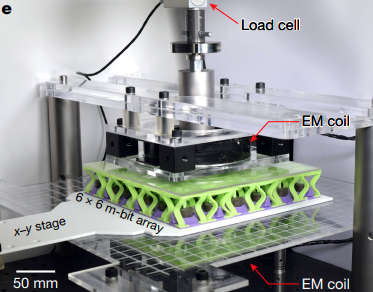
\includegraphics[scale = 0.5]{source/pictures/device.png}
        \caption{Imagem do dispositivo\cite{chen2021reprogrammable}.}
        \label{fig:device}
    \end{figure}

\subsubsection{O que é este dispositivo?}
    É um \textcolor{red}{dispositivo/sistema de memória} desenvolvido por Chen et al. capaz manipular informações de forma mecânica na estrutura do \textcolor{red}{material}\cite{coulais2021snappy}.\\ 

    Sendo capaz de:

    \begin{itemize}
        \item Codificar
        \item Armazenar
        \item Ler
        \item Alterar propriedades mecânicas do material
    \end{itemize}

    Para entendermos mais sobre este dispositivo, é necessário abordar os dois conceitos que envolvem este tema, que são: os metamateriais e os sistemas de armazenamento de dados. 

\subsection{Metamaterias}

\subsection{Sistemas de memória}
    Para melhor compreensão do funcionamento deste dispositivo, vamos construir uma analogia com outro dispositivo já conhecido que possui um funcionamento semelhante.

\subsubsection{Discos Rigidos}

    \begin{figure}[H]
        \centering
        \includegraphics[scale = 0.05]{source/pictures/hdd.png}
        \caption{Imagem de um disco rígido\cite{hdd-image}.}
        \label{fig:hdd}
    \end{figure}

    \begin{itemize}
        \item Apresenta funcionamento semelhante ao SDS\footnote{Snappy Data Storage}
        \item Utiliza \textit{bits} magneticos para manipular a informação
    
    \end{itemize}

    São sistemas de armazenamento de dados que apresentam funcionamento semelhante ao Snappy Data Storage, no entanto se baseia em um funcionamento eletromagnético para manipular as suas unidades básicas de memória, que são os bits.

\subsubsection{Funcionamento dos Discos Rígidos}

\begin{figure}[H]
    \centering
    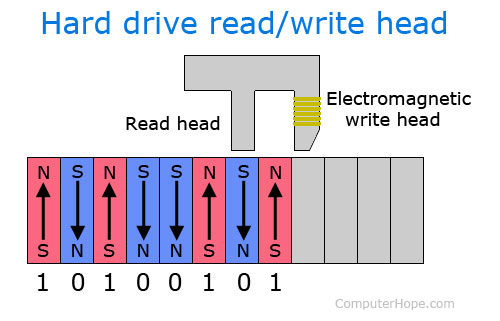
\includegraphics[scale = 0.5]{source/pictures/magnetic-media.jpg}
    \caption{Processo de gravação em um disco rígido\cite{hdd-image}.}
    \label{fig:hdd-recording}
\end{figure}

Para gravar informações em um disco rígido, o dispositivo através de um cabeçote eletromagnético magnetiza um bit e a sua polaridade determina o valor daquele bloco(\textit{building block})\cite{hdd-image}. Por exemplo, esta sequência de valores gravados significa o número 165 em código binário.\\ O bit é a unidade básica de memória deste sistemas, podendo assumir dois valores, sendo um ou zero. Este conceito será importante para entender o funcionamento do objeto de estudo deste trabalho.



\section{Funcionamento}

\subsection{Unidade Básica de Armazenamento}
\begin{figure}[H]
    \centering
    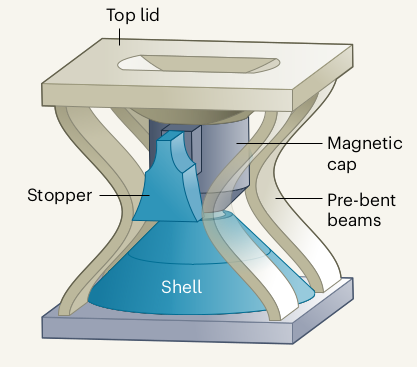
\includegraphics[scale = 0.5]{source/pictures/shell.png}
    \caption{Unidade básica de armazenamento mecânico\cite{coulais2021snappy}.}
    \label{fig:uba}
\end{figure}

A estrutura da unidade básica de armazenamento mecânica possui esta estrutura, que é projeta para ter uma instabilidade de encaixe. Ela conta com dois \textit{sttopers}, que funcionam como braços para limitar a movimentação da estrutura interna e uma tampa magnética. Através dela, é possível orientar remotamente o encaixe da estrutura, por meio de um campo magnético.


\begin{figure}[H]
    \centering
    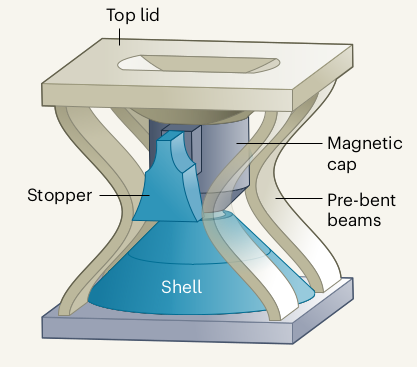
\includegraphics[scale = 0.5]{source/pictures/shell.png}
    \caption{Estados da UBA\cite{coulais2021snappy}.}
    \label{fig:uba-states}
\end{figure}

Nesta imagem(\ref{fig:uba-states}) é possível ver como a estrutura se altera conforme uma mudança na orientação magnética da tampa. A partir disso, é possível definir se o material é mais facilmente comprimido ou o contrário.

\subsection{Processo de gravação}

Semelhante ao disco rígido, onde o cabeçote eletromagnético orienta a polaridade da unidade básica de memória. Neste caso, um cabeçote eletromagnético vai ser responsável por orientar o estado da estrutura, como foi possível ver anteriormente.

\begin{center}
\textcolor{red}{\textbf{[VIDEO DE GRAVAÇÃO EM UBA]}}
\end{center}

Neste vídeo, é possível analisar a orientação do encaixe em uma unidade, a partir criação de um campo eletromagnético.

\begin{center}
\textcolor{red}{\textbf{[VIDEO DE GRAVAÇÃO EM ARRAY]}}
\end{center}


\section{Propriedades mecânicas dos bits}

Como foi visto anteriormente, gravar uma informação neste dispositivo gera uma alteração na estrutura das unidades que o compõem. No video a seguir é possível ver o comportamento de uma unidade diante de uma compressão em seus dois estados. 

\begin{center}
\textcolor{red}{\textbf{[VIDEO DE TESTE DE COMPRESSIBILIDADE DE UMA UNIDADE DE GRAVAÇÃO]}}
\end{center}
    
Agora em um material formado por estas unidades. 

\begin{center}
\textcolor{red}{\textbf{[VIDEO DE TESTE DE COMPRESSIBILIDADE EM UM MATERIAL FORMADOS POR ESTAS UNIDADES]}}
\end{center}

Desse modo, é possível ver como podemos controlar o comportamento de um material por meio da gravação de informações nele. 
\section{Resultados}

\subsection{Inovações}
Este dispositivo traz uma grande contribuição para a comunidade, pois foi o primeiro metamaterial que apresentou simultâneamente:

\begin{itemize}
    \item Bits definindo propriedades mecânicas
    \item O estado dos bits podem ser controlados remotamente
\end{itemize}

\subsection{Limitações}
Apesar de apresentar diversas inovações, o dispositivo ainda possui algumas limitações que ainda restrigem de elaborar aplicações práticas. Pois:
\begin{itemize}
    \item Geometria complexa do material
    \item Densidade de armazenamento\footnote[1]{São necessários 10mm² para obter 1 bit, obtendo 36 bits com 1080mm².}
\end{itemize}

Por ter uma geometria complexa, se tornar dificil o processo de miniaturizar estas estruturas. O que impacta no segundo ítem, que é o fato de ter uma densidade de armazenamento extremamente baixa, pois para ter um bit é necessário ter uma área de 10mm².


\section{Considerações finais}

\lipsum[1]

\begin{citacao}
    \lipsum[2]
\end{citacao}

\lipsum[3]
%//todo este section acima deve ser numerada em sequência, use um número na frente, exemplo 03.1-r-graphics.tex
%//valar erick-suzart
%//checked mhar-vell - OK
% ----------------------------------------------------------
\bookmarksetup{startatroot}% Finaliza a parte no bookmark do PDF, para que se inicie o bookmark na raiz 
% ----------------------------------------------------------
% ELEMENTOS PÓS-TEXTUAIS
% ----------------------------------------------------------
\postextual
% 
% Referências bibliográficas
% ----------------------------------------------------------
\bibliography{bibliography} 
% 
% Agradecimentos
% ----------------------------------------------------------

\end{document}
